
% Supõe-se que, na introdução, tenha sido posto a definição do problema de SQA como a necessidade de garantir um sinal de boa qualidade, seja para humanos não cometerem enganos, seja para modelos preditivos serem capazes de estimar com acurácia.

This chapter will present the state of the literature of the \acrlong{SQA} of cardiological signals problem, using a top to bottom approach, finishing on this thesis work scope. Then, this chapter will expose this work contribution.

\section{Signal Quality Assessment}

The \acrfull{SQA} challenge is not exclusive to the medical domain. Actually, its origins are related to the old comunication systems, when researchers published their first works on the theory of information in the 1920s and 1930s. One example of such works is the ``Mathematical analysis of random noise'', by Stephen O. Rice, in which he analyzes the statistical properties of comunication device noises \cite{origins-1}. Another example is the work of Claude E. Shannon, ``A mathematical theory of communication'', which introduces fundamental concepts in comunication systems \cite{origins-2}. In that millennium, studies already used the concept of \acrshort{SQA}. We can see samples of this in the 1980s, such as the work of R. H. Stehle, which proposed an algorithm for assessing the quality of shortwave broadcast signals, trying to objectively measure the human perception of the signal mensage intelligibility \cite{origins-3}. Some of its conclusions are useful in the \acrshort{SQA} in clinical contexts, such as the high degree of subjectivity in the human idea of quality. This makes labeling datasets properly fundamental to reflect this concept of quality in the proper evaluation of the developed \acrshort{SQA} algorithms.
	
Past the 20th century, the \acrshort{SQA} of physiological signals begin to become popular. Particularly, the early 2000s decade had several works in the subject. One of them is the work of \citeauthor{2000s-1}, which proposed a \acrshort{ECG} assessment method based on the difference between the areas of distinct QRS complexes \cite{2000s-1}. The work propose comparing the cummulative histograms of different \acrshort{ECG} leads to assess its qualities. Later, \citeauthor{2000s-2} suggested the combination of different quality metrics by measuring their inner and between \acrshort{ECG} lead ammount of agreement, giving one final metric \cite{2000s-2}. Another work, by \citeauthor{2000s-3}, posed the thresholding based on the Hjorth parameters to assess the quality of \acrshort{PPG} signals \cite{2000s-3}. Afterwards, \citeauthor{2000s-4} elaborated a \acrshort{ABP} signal quality assessment metric based on the End Diastole Slope Sum and Slow Ejection Slope Sum features. Through those works, researchers proposed quantifying the \acrshort{SQA} in a metric. A common name that they used to refer to this metric was \acrfull{SQI}. 


\subsection{The Signal Types}

Among the variety of physiological signals, the \acrfull{ECG} is prevalent in the literature. This signal has multiple applications, such as disease classification, heartbeat type detection, biometric detection and emotion recognition \cite{ecg-1}. There are a plenty of works in the \acrshort{SQA} of ECG signals. In one of them, \citeauthor{ecg-2} proposed two features for the estimation of a classification \acrshort{SQI} of multi-channeled \acrshort{ECG}s. One feature consists of verifying if two energy-like indices, measured in deciBels, are within an admissible range. The other feature result from randomly chosing a target lead, feeding a \acrshort{FFNN} with array of derivatives of all leads to reconstruct the targeted lead and finally comparing the original target lead to its artificial version with correlation analysis. In 2017, \citeauthor{ecg-3} introduced a feature based on the extraction of the Heart Rate Variability of \acrshort{ECG} signals. The method decomposes this new signal into wavelets with different frequency ranges and calculates the each of them entropy, forming a feature vector. This vector feed a \acrshort{SVM}, which classifies the signal as acceptable or not. Later, \citeauthor{ecg-4} developed an image-based feature that measures the Structural Similarity Measure between the input plot image, containing each signal channel cartesian graph, and multiple template plot images of similar shape selected from the training dataset by using clustering analysis. One year later, \citeauthor{ecg-5} proposed transforming the signal using the Auto Correlation Function and extracting simple features from it \cite{ecg-5}. In the current year, \citeauthor{ecg-6} generated phase space plots, such as Poincaré plots and First Order Difference graphs, and discretized them into a grid where each cell is the logarithm of the number of points contained in that cell \cite{ecg-6}. Thus, the \acrshort{SQA} literature for \acrshort{ECG} is already well developed.

However, an alternative to the \acrshort{ECG}, \acrfull{PPG}, has only increased in popularity. In fact, its number of related articles published from 2013 to 2023 has increased in 176\% \cite{ppg-1}. This signal also elevated in presence in the \acrshort{SQA} literature. A sample of this literature is the work of \citeauthor{review-1}, which poses the measurement of a \acrshort{SQI} through the application of the Dynamic Time Warping techinique \cite{review-1}. It finds the optimal path cost on a distance matrix which encodes the differences between each pair of points of the input and a template, reference of a good signal. \citeauthor{review-1} added this techinique \acrshort{SQI} to others and feeded them to a \acrshort{MLP} and to a self-made function, predicting a unique \acrshort{SQI}. Experiments on private annotations on the MIMIC II dataset resulted on the \acrshort{MLP} achieving the highest accuracy, 95.2\% \cite{review-1}. Therefore, it is possible to achieve good accuracy in the \acrshort{SQA} of \acrshort{PPG}s.      
	
In the \acrshort{SQA} literature, the \acrshort{PPG} showed to be usefull in the \acrlong{CA} identification applications. The \acrfull{CA} is the presence of an anomalous cardiac rate, such as fast, slow or irregular \acrshort{HR} moments. Its cause is abnormalities in the cardiac nervous system. This medical condition is an obstacle in the design of \acrshort{SQI}, since, in contrast to arrhythmic individuals, normal cardiac signals are periodic. Some features assume that the signal is periodic, such as the naive \acrshort{HR} estimation based on QRS complex peaks. This assumption can result in signals with arrhythmia being reject as unreliable signals, leaving those special patients undiagnosed. \citeauthor{review-5} conducted experiments on a private dataset that contains cases of \acrfull{AF}, a type or arrhythmia \cite{review-5}. In this experiment, 40 features used in previous studies fed a \acrshort{SVM}, which achieved an average accuracy superior to 94\% \cite{review-5}. That accuracy was far higher than other existing methods, which the researchers also tested \cite{review-5}. Therefore, abundant feeding a machine learning algorithm with features and training it on datasets with arrhytmia cases already present an improvement in the detection of those special cases.

In sequence, two studies adopted a similar approach to the one mentioned in the past paragraph to attack the arrhythmia problem. In the first study, \citeauthor{review-6} feeded several features to three classifiers: \acrshort{SVM}, \acrshort{K-NN} and Decision Tree \cite{review-6}. Similarly to the antecedent study, experiments on a private dataset demonstrated that the \acrshort{SVM} was the best of all classifiers and it obtained above 95\% suprassing the methods of other studies. The second study also included the \acrshort{SVM} method, but added to the experiment deep learning models \cite{review-7}. The study contemplated both 1d and 2d deep learning models, with the first recieving the raw signal and the second recieving its cartesian plot image. Experiments on private data with presence of \acrshort{AF} showed that the ResNet18 model was the best, with 98.5\% accuracy. That last study highlighted that deep learning models have the potential to supprass conventional methods even with the presence of arrythmic events. The next section will further explore the use of deep learning in the literature.  

\subsection{The Deep Learning Approach}
\label{sec:deep_learning}

As already mentioned, \acrfull{DL} has the potential to achieve a higher accuracy than feature based models, even in the context of \acrshort{CA}. On one hand, differently of hand-crafted features, \acrshort{DL} automatically extract features from the input signal, creating models that are adaptable to different dataset training contexts. Additionally, a high quality dataset can provide resources for the \acrshort{DL} model to be robust to variations on the signal conditions. On the other hand, not only it creates a black-box that does not explain the reasons why the model atributed a certain \acrshort{SQI}, but also requires large ammounts of data to proper adjust the model parameters. Depite this, \acrshort{DL} are worth exploring since it can provide the accuracy and robustness that the medical applications require. 

In this context, several studies proposed the application of \acrshort{CNN}s, one-dimensional \acrshort{DL} models. For instance, \citeauthor{review-8} applied a self-designed \acrshort{CNN} to extract a binary \acrshort{SQI} \cite{review-8}. Tests on a private dataset with data of three devices lead to 85\% F1-score for the ``Reliable'' class. Alike, \citeauthor{review-9} employed a self-made \acrshort{CNN}, but examined the effect of transfer learning as well \cite{review-9}. They conducted the experiment on three private datasets. It beggan training the model mostly on one dataset, in which it achieved an accuracy of 99.8\%. Then, for each remaining database, they fine-tuned the the model with little training and tested on it. This procedure resulted on the 93\% and 81\% accuracies on the second and third datasets, respectively. Additionally, the model trained solely on the second database scored lower, 86\%. Those results indicate that not only we can use \acrshort{CNN} to achieve high accuracy but also we can transfer its learned features over different databases to improve its performance.

However, some works go beyond the simple application of \acrshort{CNN}s. The research of \citeauthor{review-10}, per example, introduced a hybrid-model for quality assessment, which combines a \acrshort{CNN} with a rule-based approach. This rule can bypass the utilization of the \acrshort{CNN} by verifying if the signal min to max distance is less than an threshold. They determined the threshold by methods such as Last Value Thresholding and Nearest Value Thresholding. The researchers did it to avoid the unecessary power usage by the \acrshort{DL} model. The method proved to be functional since it avoided the usage of the \acrshort{CNN} for 3.27\% of the input samples, while mantaining similar prediction scores if compared to the \acrshort{CNN} without the rule component \cite{review-10}. Therefore, we can achieve particular advantages by combining the \acrshort{CNN} with other methods.  

Besides \acrshort{CNN}s, works explored the use of alternative \acrshort{DL} models such as recurrent networks. \citeauthor{review-11} proposed the application of a Long Short-Term Memory network for real time \acrshort{SQA}, giving a \acrshort{SQI} for each point in the signal. For the experiments, they labeled private and public datasets by applying Blind Source Separation to generate from each \acrshort{PPG} signal one high-quality signal and one low-quality signal. When compared to baseline \acrshort{SQI}s and existing models, it achieved competitive accuracy, while being lightweighted and enoughly fast to predict in real-time \cite{review-11}. Therefore, recurrent networks can suit well for real-time \acrshort{SQA} tasks.

Additionally, other researchers proposed the application of 2D \acrshort{CNN}s. One of those, \citeauthor{review-12}, proposed, initially, the transformation of the input signal into a Short-Time Fourier Transform spectogram. Then, this image feeds a 2D \acrshort{CNN} which classifies the quality of the signal. The researchers annotated the VitalDB database and, then, conducted experiments that lead to the proposed method achieving a better accuracy than four chosen baseline models. Its value was 98,3\%. Therefore, transforming the input into a image can result in improved accuracy. The next section will explore the time series imaging scope of the \acrshort{SQA} literature.


\newcommand{\projectionsWidth}{0.2\textwidth}

\begin{figure}[h]
    	\centering
%    \bgroup
%    \setlength{\tabcolsep}{1mm}
%    \def\arraystretch{2}
%    \adjustbox{max width=0.92\textwidth}{%
%    \begin{tabular}{cccc}
%    \multicolumn{4}{c}{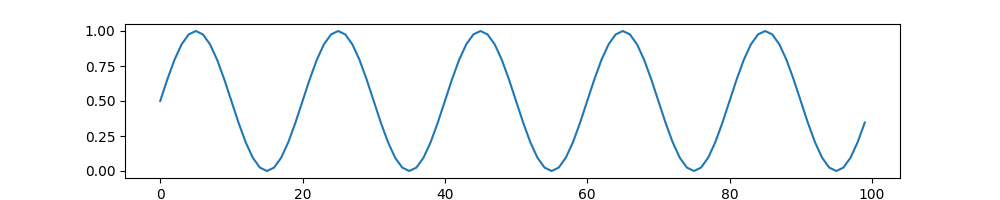
\includegraphics[width=0.95\textwidth, trim={2cm 0cm 2cm 0cm}]{img/projections/signal.png}} \\
%        \fbox{
\includegraphics[width=\projectionsWidth]{img/projections/GramianAngularFieldDifference.png}}
%         & \fbox{
\includegraphics[width=\projectionsWidth]{img/projections/GramianAngularFieldSummation.png}}
%         & \fbox{
\includegraphics[width=\projectionsWidth]{img/projections/MarkovTransitionField.png}}
%         & \fbox{
\includegraphics[width=\projectionsWidth]{img/projections/RecurrencePlot.png}}\\
%        \fbox{
\includegraphics[width=\projectionsWidth]{img/projections/PoincatePlotLogarithmGrid.png}}
%        & \fbox{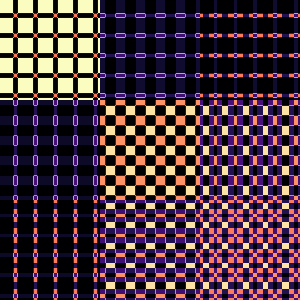
\includegraphics[width=\projectionsWidth]{img/projections/MultiscaleMarkovTransitionField.png}}
%        & \fbox{
\includegraphics[width=\projectionsWidth, height=\projectionsWidth]{img/projections/ShortTimeFFT.png}}
%        & ~ \\
%    \end{tabular}
%    }
%    \egroup
%   	\caption[A signal and its various projection obtained by several methods.]{A signal and its various projection obtained by several methods. In the first line, from the left to the right, the methods are: Gramian Angular Diference Field~\cite{gaf-mtf-1}, Gramian Angular Summation Field~\cite{gaf-mtf-1}, Markov Transition Field~\cite{gaf-mtf-1} and Recurrence Plot~\cite{rp-1}. The methods of the second line are, from the left to the right: Poincaré Plot Density Map~\cite{ecg-6}, Multiscale Markov Transition Field~\cite{imaging-6} and Short Time Fourier Transform Spectogram~\cite{STFT, imaging-1}.}
	\subfigure[]{
		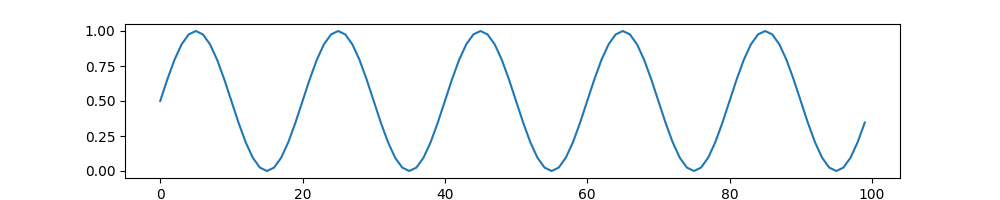
\includegraphics[width=0.95\textwidth]{img/projections/signal.png}
		\label{fig:projections:signal}
	}\\
	\subfigure[]{
		
\includegraphics[width=\projectionsWidth]{img/projections/GramianAngularFieldDifference.png}
		\label{fig:projections:GramianAngularFieldDifference}
	}
	\subfigure[]{
		
\includegraphics[width=\projectionsWidth]{img/projections/GramianAngularFieldSummation.png}
		\label{fig:projections:GramianAngularFieldSummation}
	}
	\subfigure[]{
		
\includegraphics[width=\projectionsWidth]{img/projections/MarkovTransitionField.png}
		\label{fig:projections:MarkovTransitionField}
	}
	\subfigure[]{
		
\includegraphics[width=\projectionsWidth]{img/projections/RecurrencePlot.png}
		\label{fig:projections:RecurrencePlot}
	}\\
	\subfigure[]{
		
\includegraphics[width=\projectionsWidth]{img/projections/PoincatePlotLogarithmGrid.png}
		\label{fig:projections:PoincatePlotLogarithmGrid}
	}
	\subfigure[]{
		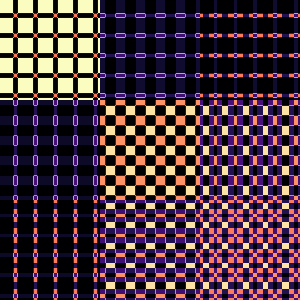
\includegraphics[width=\projectionsWidth]{img/projections/MultiscaleMarkovTransitionField.png}
		\label{fig:projections:MultiscaleMarkovTransitionField}
	}
	\subfigure[]{
		
\includegraphics[width=\projectionsWidth]{img/projections/ShortTimeFFT.png}
		\label{fig:projections:ShortTimeFFT}
	}\\
   	\caption[A signal and its various projection obtained by several methods.]{
   		A signal~\subref{fig:projections:signal} and its various projection obtained by several methods. They are: 
   		\subref{fig:projections:GramianAngularFieldDifference}~Gramian Angular Diference Field~\cite{gaf-mtf-1}, 
   		\subref{fig:projections:GramianAngularFieldSummation}~Gramian Angular Summation Field~\cite{gaf-mtf-1}, 
   		\subref{fig:projections:MarkovTransitionField}~Markov Transition Field~\cite{gaf-mtf-1} and 
   		\subref{fig:projections:RecurrencePlot}~Recurrence Plot~\cite{rp-1}, 
   		\subref{fig:projections:PoincatePlotLogarithmGrid}~Poincaré Plot Density Map~\cite{ecg-6}, 
   		\subref{fig:projections:MultiscaleMarkovTransitionField}~Multiscale Markov Transition Field~\cite{imaging-6} and 
   		\subref{fig:projections:ShortTimeFFT}~Short Time Fourier Transform Spectogram~\cite{STFT, imaging-1}.
   	}
    	\label{fig:literature_projections}
\end{figure}



\subsection{The Time Series Imaging Techinique}
\label{sec:imaging}

Several works in the literature propose transforming the input signal into a image and, then, feeding it to a computer vision model. The figure \ref{fig:literature_projections} shows some of those transformations. The works that this paragraph mentions all used \acrshort{CNN}s as a classifier of the \acrshort{SQI}. \citeauthor{review-13} transformed the signal into Quantum Pattern Recognition images for PPG \acrshort{SQA}. This resulted in 98,3\% accuracy on the University of Queensland vital signs dataset with labels from the researchers, scoring above baseline models and an existing \acrshort{DL} method \cite{review-13}. \citeauthor{review-15} embeded the signal into a Recurrence Plot matrix for PPG \acrshort{SQA}. On a private datset, the method achieved 97,5\% accuracy \cite{review-15}. Therefore, the application of time series image proved to be effective in the \acrshort{SQA} literature.  

One particular method present in the \acrshort{SQA} literature is the time series matrix embedding, which encodes time relationships of the original signal into a square matrix. For instance, \citeauthor{review-16} feeded a Vision Transformer with a Recurrence Plot or a Markov Transition Field, achieving, respectivelly, 89,9\% and 90,3\% accuracy on a private dataset \cite{review-16}. \citeauthor{review-17} also feeded images with a Vision Transformer, but used Gramian Angular Fields. The proposed approach reached 92,2\% accuracy on a private dataset \cite{review-17}. \citeauthor{review-18} proposed the use of Multiscale Markov Transition Fields, version which concatenates the signal first and second derivatives. This projection feeded a self-made computer vision model. Experiments with pre-training on the MIMIC-III and UCI databases, and fine-tuning and testing on the Queensland dataset resulted in 99,1\% accuracy for binary classification \cite{review-18}. Thus, the combination of a generic computer vision model with a projection method, such as Recurrence Plot, Gramian Angular Field or Markov Transition Field, can achieve a decent accuracy, while it is possible to apply the multiscaling techinique to improve some of those projections accuracy. 

\section{This work contribution}
\label{sec:my_work}

This section will explain this work contribution. Firstly, this work proposes a new and effective approach for encoding time series. It aggregates different projections into a composite hyperspectral image. This aggregation showed to be better than using one of the projections methods alone. Secondly, this work also evaluates the proposed approach in combination with a great ammount of computer vision models, which none of the above-mentioned works did. That gives insights on which types of models are ideal for the time series matrix embedding techinique. Thirdly, this thesis also attemp a novel idea of transfer learning with source in a dataset out of the \acrshort{SQA} domain, in this case, the ImageNet dataset. That has the potential to reduce the need of a large ammount of labeled \acrshort{PPG} data. Finally, this thesis did experiments on a publicly avalliable and labeled dataset, \acrfull{BUTPPG}, which ensures the reproductibility and comparability of this work experiment. The lack of reproductibility was a noticeable problem in the literature that this chapter reviewed.     
